\documentclass[11pt,twocolumn,oneside,openany,headings=optiontotoc,11pt,numbers=noenddot]{article}

\usepackage[a4paper]{geometry}
\usepackage[utf8]{inputenc}
\usepackage[T1]{fontenc}
\usepackage{lmodern}
\usepackage[ngerman]{babel}
\usepackage{ngerman}

\usepackage[onehalfspacing]{setspace}

\usepackage{fancyhdr}
\usepackage{fancybox}

\usepackage{rotating}
\usepackage{varwidth}

%Struktogramme
\usepackage[german,curves]{struktex}

\usepackage{pdflscape}
\usepackage{changepage}
\usepackage{graphicx}
\usepackage[bottom]{footmisc}
\usepackage{transparent}
\usepackage{graphbox}
\graphicspath{
	{Pics/PDFs/}
	{Pics/JPGs/}
	{Pics/PNGs/}
}
\usepackage{caption}
\usepackage{wrapfig}
\usepackage{marginnote}
\usepackage{tabularx}
\usepackage{dashrule}
\usepackage{soulutf8}
\usepackage{hhline}
%arydshln suppresses vertical lines in table
%\usepackage{arydshln}
\usepackage{multirow}
\usepackage{enumerate}
\usepackage[hidelinks]{hyperref}
\usepackage{listings}

\usepackage[table]{xcolor}
\usepackage{array}
\usepackage{enumitem,amssymb,amsmath}
\usepackage{interval}
\usepackage{cancel}
\usepackage{stmaryrd}
\usepackage{wasysym}
\usepackage{polynom}
\usepackage{diagbox}
\usepackage{dashrule}
\usepackage{framed}
\usepackage{mdframed}
\usepackage{karnaugh-map}
\usepackage{pdfpages}

\usepackage{blindtext}

\usepackage{eso-pic}

\usepackage{amssymb}
\usepackage{eurosym}

\usepackage[pages=some]{background}
\pagestyle{headings}
\renewcommand{\headrulewidth}{0.2pt}
\renewcommand{\footrulewidth}{0.2pt}
\newcommand*{\underdownarrow}[2]{\ensuremath{\underset{\overset{\Big\downarrow}{#2}}{#1}}}
\setlength{\fboxsep}{5pt}
\newcommand{\explainBelow}[3]{\underbrace{#1}_{\parbox{\widthof{#3}}{\footnotesize\raggedright #2}}}
\newcommand{\explainAbove}[3]{\overbrace{#1}^{\parbox{\widthof{#3}}{\footnotesize\raggedright #2}}}
\newcommand\footnoteref[1]{\protected@xdef\@thefnmark{\ref{#1}}\@footnotemark}


% Codestyle defined
\definecolor{codegreen}{rgb}{0,0.6,0}
\definecolor{codegray}{rgb}{0.5,0.5,0.5}
\definecolor{codepurple}{rgb}{0.58,0,0.82}
\definecolor{backcolour}{rgb}{0.95,0.95,0.92}
\definecolor{deepgreen}{rgb}{0,0.5,0}
\definecolor{darkblue}{rgb}{0,0,0.65}
\definecolor{mauve}{rgb}{0.40, 0.19,0.28}
\colorlet{exceptioncolour}{yellow!50!red}
\colorlet{commandcolour}{blue!60!black}
\colorlet{numpycolour}{blue!60!green}
\colorlet{specmethodcolour}{violet}

%Neue Spaltendefinition
\newcolumntype{L}[1]{>{\raggedright\let\newline\\\arraybackslash\hspace{0pt}}m{#1}}
\newcolumntype{M}{>{\centering\arraybackslash}X}
\newcommand{\cmnt}[1]{\ignorespaces}
%Textausrichtung ändern
\newcommand\tabrotate[1]{\rotatebox{90}{\raggedright#1\hspace{\tabcolsep}}}

%Intervall-Konfig
\intervalconfig {
	soft open fences
}

%Bash
\lstdefinestyle{BashInputStyle}{
	language=bash,
	basicstyle=\small\sffamily,
	backgroundcolor=\color{backcolour},
	columns=fullflexible,
	backgroundcolor=\color{backcolour},
	breaklines=true,
}
%Java
\lstdefinestyle{JavaInputStyle}{
	language=Java,
	backgroundcolor=\color{backcolour},
	aboveskip=1mm,
	belowskip=1mm,
	showstringspaces=false,
	columns=flexible,
	basicstyle={\footnotesize\ttfamily},
	numberstyle={\tiny},
	numbers=none,
	keywordstyle=\color{purple},,
	commentstyle=\color{deepgreen},
	stringstyle=\color{blue},
	emph={out},
	emphstyle=\color{darkblue},
	emph={[2]rand},
	emphstyle=[2]\color{specmethodcolour},
	breaklines=true,
	breakatwhitespace=true,
	tabsize=2,
}
%Python
\lstdefinestyle{PythonInputStyle}{
	language=Python,
	alsoletter={1234567890},
	aboveskip=1ex,
	basicstyle=\footnotesize,
	breaklines=true,
	breakatwhitespace= true,
	backgroundcolor=\color{backcolour},
	commentstyle=\color{red},
	otherkeywords={\ , \}, \{, \&,\|},
	emph={and,break,class,continue,def,yield,del,elif,else,%
		except,exec,finally,for,from,global,if,import,in,%
		lambda,not,or,pass,print,raise,return,try,while,assert},
	emphstyle=\color{exceptioncolour},
	emph={[2]True,False,None,min},
	emphstyle=[2]\color{specmethodcolour},
	emph={[3]object,type,isinstance,copy,deepcopy,zip,enumerate,reversed,list,len,dict,tuple,xrange,append,execfile,real,imag,reduce,str,repr},
	emphstyle=[3]\color{commandcolour},
	emph={[4]ode, fsolve, sqrt, exp, sin, cos, arccos, pi,  array, norm, solve, dot, arange, , isscalar, max, sum, flatten, shape, reshape, find, any, all, abs, plot, linspace, legend, quad, polyval,polyfit, hstack, concatenate,vstack,column_stack,empty,zeros,ones,rand,vander,grid,pcolor,eig,eigs,eigvals,svd,qr,tan,det,logspace,roll,mean,cumsum,cumprod,diff,vectorize,lstsq,cla,eye,xlabel,ylabel,squeeze},
	emphstyle=[4]\color{numpycolour},
	emph={[5]__init__,__add__,__mul__,__div__,__sub__,__call__,__getitem__,__setitem__,__eq__,__ne__,__nonzero__,__rmul__,__radd__,__repr__,__str__,__get__,__truediv__,__pow__,__name__,__future__,__all__},
	emphstyle=[5]\color{specmethodcolour},
	emph={[6]assert,range,yield},
	emphstyle=[6]\color{specmethodcolour}\bfseries,
	emph={[7]Exception,NameError,IndexError,SyntaxError,TypeError,ValueError,OverflowError,ZeroDivisionError,KeyboardInterrupt},
	emphstyle=[7]\color{specmethodcolour}\bfseries,
	emph={[8]taster,send,sendMail,capture,check,noMsg,go,move,switch,humTem,ventilate,buzz},
	emphstyle=[8]\color{blue},
	keywordstyle=\color{blue}\bfseries,
	rulecolor=\color{black!40},
	showstringspaces=false,
	stringstyle=\color{deepgreen}
}

\lstset{literate=%
	{Ö}{{\"O}}1
	{Ä}{{\"A}}1
	{Ü}{{\"U}}1
	{ß}{{\ss}}1
	{ü}{{\"u}}1
	{ä}{{\"a}}1
	{ö}{{\"o}}1
}

% Neue Klassenarbeits-Umgebung
\newenvironment{worksheet}[3]
% Begin-Bereich
{
	\newpage
	\sffamily
	\setcounter{page}{1}
	\ClearShipoutPicture
	\AddToShipoutPicture{
		\put(55,761){{
				\mbox{\parbox{385\unitlength}{\tiny \color{codegray}BBS I Mainz, #1 \newline #2
						\newline #3
					}
				}
			}
		}
		\put(455,761){{
				\mbox{\hspace{0.3cm}
\includegraphics[width=0.2\textwidth]{../../logo.pdf}}
			}
		}
	}
}
% End-Bereich
{
	\clearpage
	\ClearShipoutPicture
}

\setlength{\columnsep}{3em}
\setlength{\columnseprule}{0.5pt}

\geometry{left=2.50cm,right=2.50cm,top=3.00cm,bottom=1.00cm,includeheadfoot}
\pagenumbering{gobble}
\pagestyle{empty}

\begin{document}
	\begin{worksheet}{BGY 16}{Klassenstufe 13 - Mathematik}{Lernabschnitt 1: Natürliche Exponentialfunktionen und verknüpfte Exponentialfunktionen}
		
		\section{Die Grundlagen in der Übersicht}
		Wachstumsmodelle wie z.B. \glqq{}beschränktes Wachstum\grqq{} im Vergleich zu ganzrationalen Funktionen haben den Vorteil, dass sie eine Schranke aufweisen.\\
		Allerdings wissen wir bisher noch nicht genau, wie wir Änderungen im Steigungsverhalten bzw. Krümmungsverhalten abbilden können.\\
		Möglich wird beides dadurch, dass wir die natürliche Exponentialfunktion mit einer ganzrationalen Funktion (\(a_nx^n + a_{n-1}x^{n-1}\ldots{}+a_1x + a_0\)) bzw. addiert.\\
		\par\noindent
		\textit{Beispiel:}\\
		\textit{Die Entwicklung einer Medikamentenkonzentration im Blut eines Patienten wird durch folgende Funktion dargestellt.}\\
		\par\noindent
		\begin{tabularx}{0.48\textwidth}{Xl}
			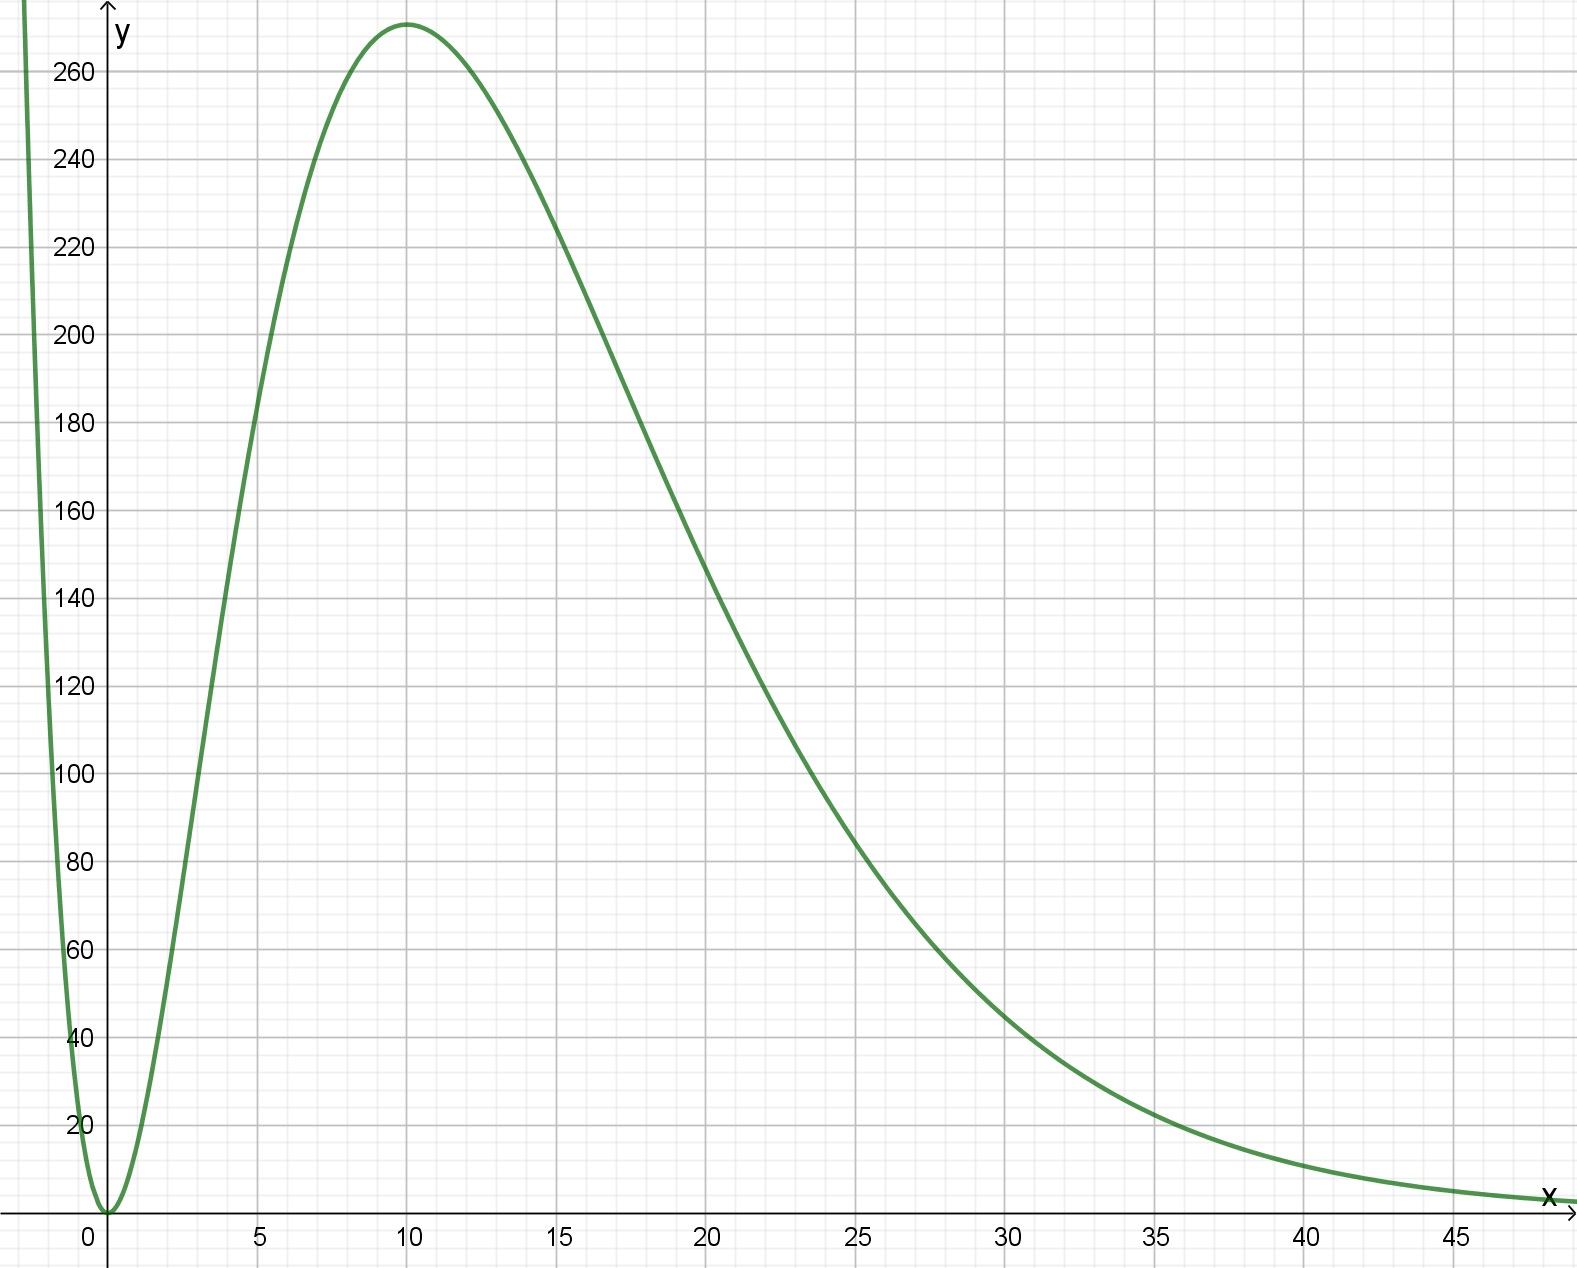
\includegraphics[width=0.38\textwidth,align=c]{../99_Bilder/01_ExpFkt/BspSkript_01.jpg} & \(f(x) = 20x^2\cdot{}e^{-0,2x}\)
		\end{tabularx}\\
		\subsection{Eine e-Funktion als Faktor: \underline{Die Produktregel}}
		Hat der Funktionsterm die Struktur \glqq{}\textit{e-Funktion$\cdot$Ganzrationale Funktion}\grqq{} (z.B. \(f(x) = 20x^2\cdot{}e^{-0,2x}\)) wird beim Ableiten die Produktregel angewandt.\\
		\par\noindent
		\begin{framed}
			\noindent
			Formel (\small{Produktregel}\normalsize): \(f(x) = u(x)\cdot{}v(x)\)\\
			\par\noindent
			$\Rightarrow$\\
			
\includegraphics[width=0.05\textwidth]{../../empty.jpg}
		\end{framed}
		\noindent
		\underline{\textit{Beispiel:}} Wenden Sie die Produktregel auf folgende Funktion an: \(f(x) = 20x\cdot{}e^{-0,2x}\)\\
		Geben Sie sowohl \(u(x)\) wie auch \(v(x)\) an.\\
		
\includegraphics[width=0.1\textwidth]{../../empty.jpg}
		\subsection{Nullstellenberechnung nach der Produktregel}
		Da Extremstellen von \(f\) Nullstellen bei \(f'\) sind, muss man also Nullstellen der ersten Ableitung bestimmen können.\\
		Dies geschieht mittels \textbf{Faktorisieren} (FAK) - ausklammern der gemeinsamen Faktoren - und anschließendem anwenden der Regel \grqq{}\textit{Ein Produkt nimmt den Wer Null an, wenn ein Faktor den Wert Null annimmt.}\grqq{}(PIN)\\
		\par\noindent
		\underline{\textit{Beispiel}:} Faktorisieren Sie die folgende Gleichung und lösen im Anschluss unter Verwendung der PIN-Regel!
		\[0 = 40x\cdot{}e^{-0,2x} + 20x^2\cdot(-0,2)\cdot{}e^{-0,2x}\]
		
\includegraphics[width=0.3\textwidth]{../../empty.jpg}
		\subsection{Eine e-Funktion als Summand: \underline{Die Summenregel}}
		Hat der Funktionsterm die Struktur \grqq{}\textit{e-Funktion + Ganzrationale Funktion}\grqq{} (z.B. \(f(x) = 10x + e^{-0,5x}\)) wird beim Ableiten die Summenregel angewandt.\\
		\par\noindent
		\begin{framed}
			\noindent
			Formel (\small{Summenregel}\normalsize): \(f(x) = u(x) + v(x)\)\\
			\par\noindent
			$\Rightarrow$\\
			
\includegraphics[width=0.05\textwidth]{../../empty.jpg}
		\end{framed}
		\noindent
		\underline{\textit{Beispiel:}} Wenden Sie die Summenregel auf folgende Funktion an: \(f(x) = 10x + e^{-0,5x}\)\\
		Geben Sie sowohl \(u(x)\) wie auch \(v(x)\) an.\\
		
\includegraphics[width=0.2\textwidth]{../../empty.jpg}
		\subsection{Nullstellenberechnung nach der Summenregel}
		Wie auch schon nach der Produktregel erwähnt, geben uns die Nullstellen der ersten Ableitung \(f'\) Auskunft über die Extremstellen der Ausgangsfunktion \(f\). Nach Anwendung der Summenregel müssen wir lediglich die Gleichung \(0 = \ldots{} + e^{\ldots{}x}\) in die Form \textit{feste Zahl} \(= e^{\ldots{}x}\) transformieren. Im Anschluss können wir den \underline{natürlichen Logarithmus} verwenden, um an den Wert des Exponenten zu gelangen.\\
		\par\noindent
		\underline{\textit{Beispiel}:} Bestimmen Sie die Nullstelle der Ableitung - also:
		\[0 = 10+ (-0,5)\cdot{}e^{-0,5x}\]
		
\includegraphics[width=0.1\textwidth]{../../empty.jpg}
		\subsection{Die Kettenregel}
		Nun können wir Exponentialfunktionen der Form \(f(x) = b\cdot{}^{c\cdot{}x}\) ableiten. Hier gilt: \fbox{\(f'(x) = b\cdot{}c\cdot{}e^{c\cdot{}x}\)}.\\
		Wir verallgemeinern diese Darstellung zu \(f(x) = b\cdot{}e^{u(x)}\). In \(u(x)\) kann ein beliebiger Ausdruck mit \grq{}\(x\)\grq{} als Exponent eingesetzt werden (z.B. \(x^2\) oder \(x^2-2\)).\\
		Es gilt dann folgendes:
		\begin{framed}
			\noindent
			Ist \(f(x) = b\cdot{}e^{u(x)}\), so gilt: \[f'(x) = b\cdot{}u'(x)\cdot{}e^{u(x)}\]
		\end{framed}
		\noindent
		\underline{\textit{Beispiel}:} Bestimmen Sie die Ableitung der folgenden Funktion. Bestimmen Sie dafür zunächst \(u(x)\) und \(u'(x)\).\\
		\(f(x) = e^{2x^2+1}\)
	\end{worksheet}
\end{document}